\section{Introduction}

Offline-to-online reinforcement learning (RL) promises to reduce online sample cost by first learning from a fixed replay dataset and then fine-tuning through environment interaction. This setup is attractive for course-project-scale empirical work because it exposes a concrete tradeoff: the offline dataset can provide a useful initialization, but low-quality replay data can also bias or constrain the learned policy.

The central question in this project is:

\begin{quote}
Under low-quality replay data, how do different forms of conservatism and regularization affect offline-to-online fine-tuning?
\end{quote}

The larger course project is organized into three tracks. A-line studies value conservatism, such as CQL-family methods. B-line provides a normal or non-conservative contrast, such as PPO, SAC, or vanilla TD3-style online fine-tuning. C-line studies policy and behavior regularization, including TD3+BC, ReBRAC, SSAR, and our ATLAS mechanism probe. This draft reports the completed C-line evidence and keeps A/B-line rows as merge placeholders rather than paper-level contributions.

\todobox{A-line owner: confirm the exact value-conservatism method names and implementation source.}
\todobox{B-line owner: confirm whether the non-conservative contrast is PPO, SAC, vanilla TD3-style fine-tuning, or a combination.}

\begin{figure}[t]
\centering
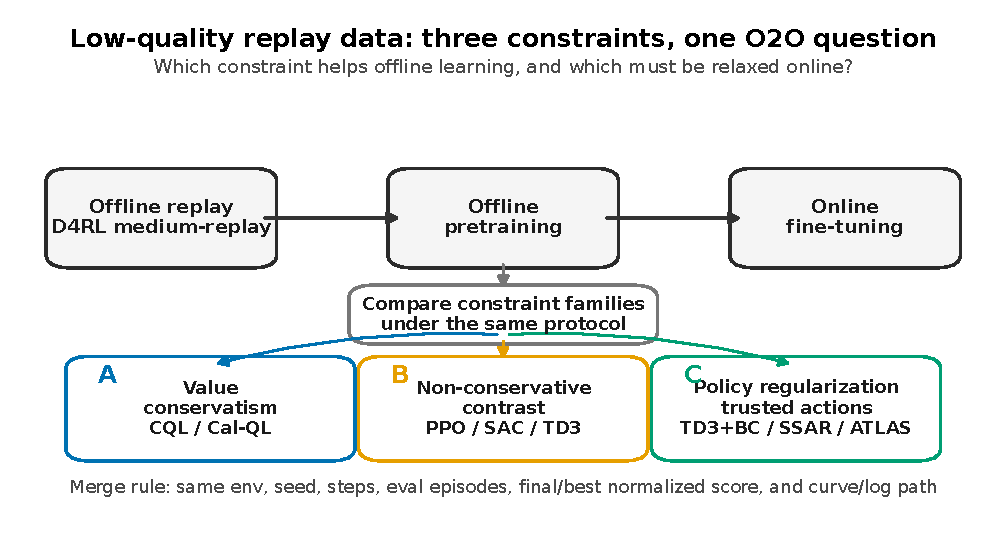
\includegraphics[width=\linewidth]{../figures/fig1_project_story.pdf}
\caption{Project framing. The final report compares three constraint families under one offline-to-online question.}
\label{fig:project-story}
\end{figure}

The current draft is written before A/B-line results are complete. Therefore, the filled evidence mainly comes from C-line. These results are already informative. On \texttt{hopper-medium-replay-v2}, simple TD3+BC is weak, stronger behavior regularization helps, and SSAR is a strong teacher. More importantly, SSAR's advantage appears tied to trusted-action selection rather than generic regularization. This motivates ATLAS, a lightweight selector that distills trusted-action labels from a cached SSAR/IQL-qv teacher into a reusable trust score. The eval20 online panel then reveals the main tension: a constraint that is useful during offline learning can become harmful during online fine-tuning. In our short O2O slice, TD3+BC improves from 22.20 to 40.06, while ATLAS and SSAR/IQL-qv teacher labels reach stronger offline endpoints but finish below that TD3+BC online final.

Our current contributions are:

\begin{enumerate}[leftmargin=*]
  \item Mechanism evidence that trusted-action selection is a high-value component of behavior-regularized offline RL under low-quality replay.
  \item ATLAS, a C-line mechanism probe showing that aligned teacher trust labels can improve offline initialization while shuffled or random trust controls fail.
  \item A cautionary offline-to-online finding: stronger teacher-label constraints can produce better offline endpoints but worse online final scores, exposing a constraint-transfer gap.
\end{enumerate}

\todobox{Final editor: after A/B-line results arrive, decide whether to restore a cross-line contribution. Until then, keep the paper framed as a C-line mechanism study.}
